\documentclass[12pt, twoside]{article}
\usepackage[letterpaper, margin=1in, headsep=0.5in]{geometry}
\usepackage[english]{babel}
\usepackage[utf8]{inputenc}
\usepackage{amsmath}
\usepackage{amsfonts}
\usepackage{amssymb}
\usepackage{tikz}
\usetikzlibrary{quotes, angles}
\usepackage{graphicx}
\usepackage{enumitem}
\usepackage{multicol}

\newif\ifmeta
\metatrue %print standards and topics tags

\title{Regents Geometry}
\author{Chris Huson}
\date{December 2021}

\usepackage{fancyhdr}
\pagestyle{fancy}
\fancyhf{}
\renewcommand{\headrulewidth}{0pt} % disable the underline of the header
\raggedbottom

\fancyhead[LE]{\thepage}
\fancyhead[RO]{\thepage \\ Name: \hspace{4cm} \,\\}
\fancyhead[LO]{BECA / Dr. Huson / Geometry 6 Trigonometry}

\begin{document}

\subsubsection*{6.5 Classwork: Tangent function, slope \hfill CCSS.HSG.SRT.C.8}
\begin{enumerate}
\item Do Now: A vector from the origin $\overrightarrow{OA}$ is shown rotated counterclockwise around $O$.
  \begin{multicols}{2}
        \begin{enumerate}
        \item Using a protractor, measure the angle of rotation.
        \item Write down the slope of $\overrightarrow{OA'}$.
        \item Mark and label the point $B(4,-3)$. Draw $\overrightarrow{OB}$.
        \item Write down the slope of $\overrightarrow{OB}$.
        \item What is the product of the slopes of $\overrightarrow{OA'}$ and $\overrightarrow{OB}$?
      \end{enumerate}
      \begin{center}
      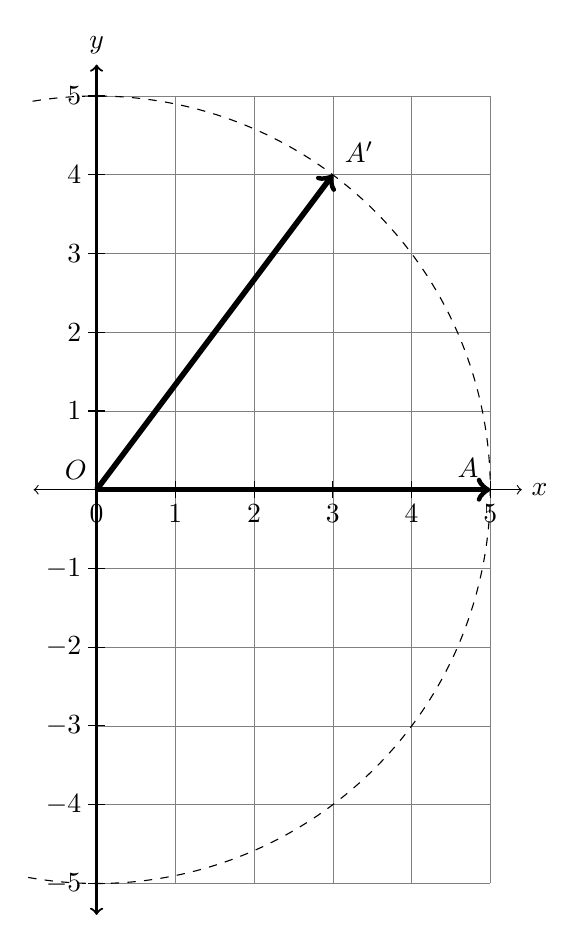
\begin{tikzpicture}[scale=1]
      \draw [help lines] (0,-5) grid (5,5);
      \draw [<->] (-0.8,0) -- (5.4,0) node [right] {$x$};
      \draw [thick, <->] (0,-5.4)--(0,5.4) node [above] {$y$};
      \foreach \x in {0,1,2,3,4,5}
        \draw[shift={(\x,0)},color=black] (0pt,-3pt) -- (0pt,3pt) node[below=5pt]  {$\x$};
      \foreach \y in {-5,...,-1,1,2,3,4,5}
        \draw[shift={(0,\y)},color=black] (-3pt,0pt) -- (3pt,0pt) node[left=5pt]  {$\y$};
      %\draw [dashed] (0,0) circle [radius=5cm];
      \draw [dashed] (-100:5) arc (-100:100:5);
      \node at (0,0)[above left]{$O$};
      \draw [line width=2pt, ->] (0,0)--(5,0) node [above left] {$A$};
      \draw [line width=2pt, ->] (0,0)--(3,4) node [above right] {$A'$};
    \end{tikzpicture}
  \end{center}
\end{multicols}

\item Complete the table mapping angle of rotation onto slope. (six entries)\\
      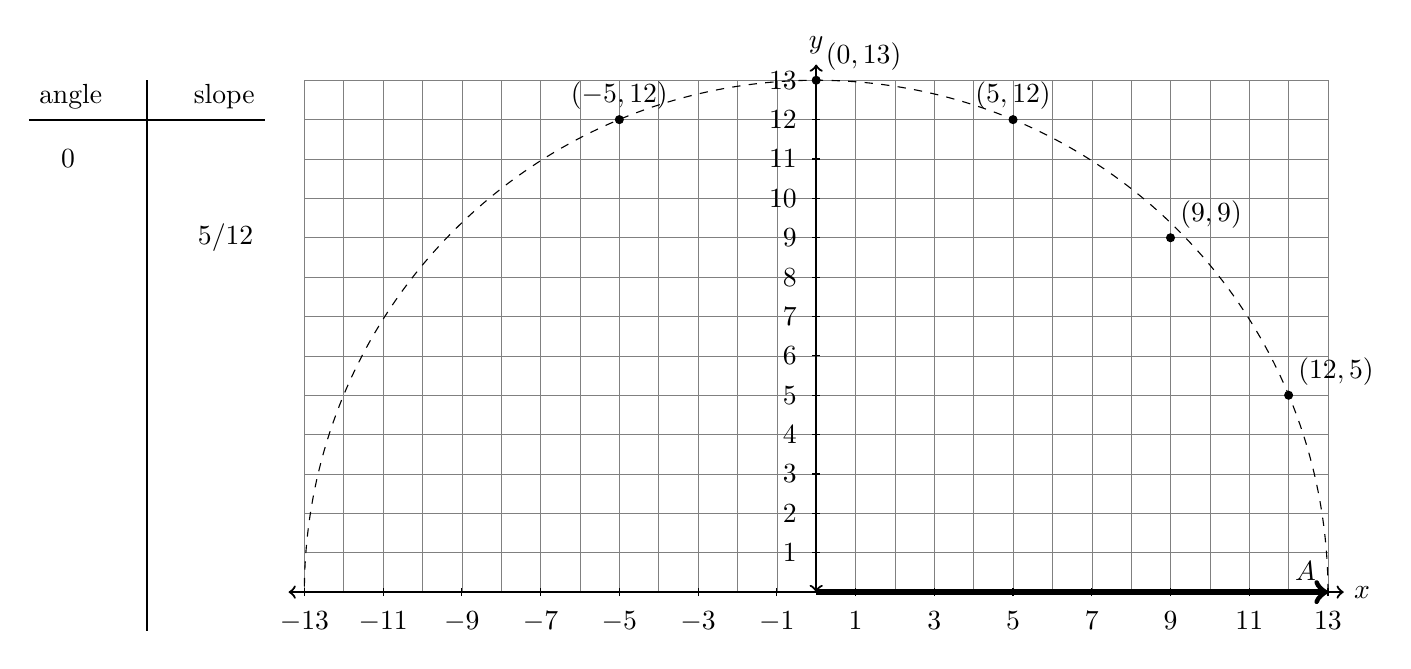
\begin{tikzpicture}[scale=0.5]
      \draw [help lines] (-13,0) grid (13,13);
      \draw [thick, <->] (-13.4,0) -- (13.4,0) node [right] {$x$};
      \draw [thick, <->] (0,0)--(0,13.4) node [above] {$y$};
      \foreach \x in {-13,-11,...,13}
        \draw[shift={(\x,0)},color=black] (0pt,-3pt) -- (0pt,3pt) node[below=5pt]  {$\x$};
      \foreach \y in {1,...,13}
        \draw[shift={(0,\y)},color=black] (-3pt,0pt) -- (3pt,0pt) node[left=5pt]  {$\y$};
      %\draw [dashed] (0,0) circle [radius=5cm];
      \draw [dashed] (0:13) arc (0:180:13);
      \draw [line width=2pt, ->] (0,0)--(13,0) node [above left] {$A$};
      \draw [fill] (12,5) circle [radius=0.1cm] node[above right]{$(12,5)$};
      \draw [fill] (5,12) circle [radius=0.1cm] node[above]{$(5,12)$};
      \draw [fill] (-5,12) circle [radius=0.1cm] node[above]{$(-5,12)$};
      \draw [fill] (9,9) circle [radius=0.1cm] node[above right]{$(9,9)$};
      \draw [fill] (0,13) circle [radius=0.1cm] node[above right]{$(0,13)$};

      \draw [thick] (-20,12) node [above right] {angle} -- (-14,12) node [above left] {slope};
      \draw [thick] (-17,13)--(-17,-1);
      \node at (-19,11){$0$};
      \node at (-15,9){$5/12$};
    \end{tikzpicture}

\newpage
  \item Use a calculator. Express the result to the nearest thousandth.\vspace{.5cm}
    \begin{multicols}{2}
      \begin{enumerate}
        \item $\tan 45^\circ = $ \vspace{1cm}
        \item $\tan 30^\circ =$
        \item $\tan 15^\circ = $ \vspace{1cm}
        \item $\tan 65^\circ =$
      \end{enumerate}
    \end{multicols} \vspace{0.5cm}

    \item \begin{enumerate}
      \item Graph and label $\triangle ABC$ with $A(0,0)$, $B(7,4)$, and $C(7,0)$.
      \begin{center}
        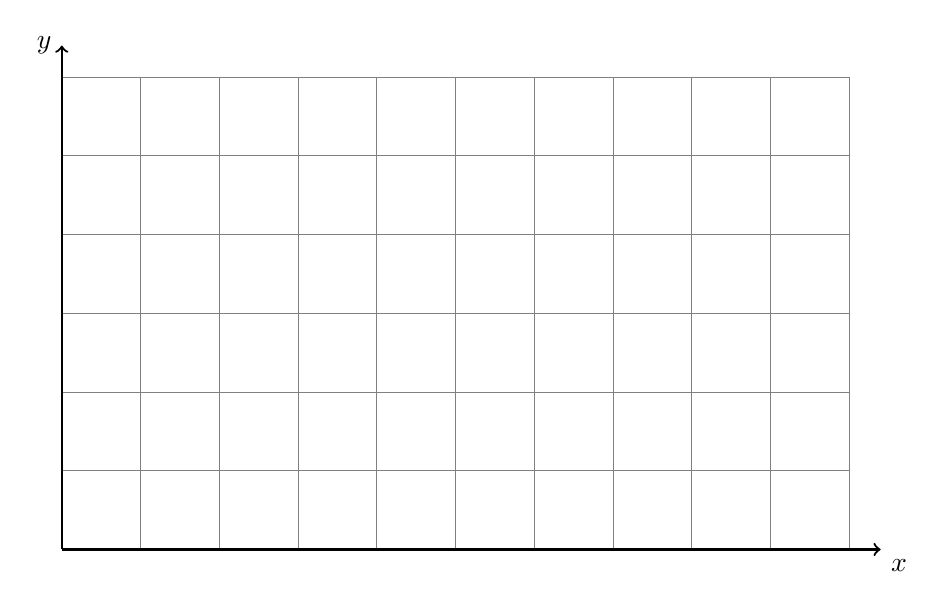
\begin{tikzpicture}%[scale=.635]
          \draw [help lines] (0,0) grid (10,6);
          \draw [thick, ->] (0,0) -- (10.4,0) node [below right] {$x$};
          \draw [thick, ->] (0,0)--(0,6.4) node [left] {$y$};
        \end{tikzpicture}
      \end{center}
      \item Find the slope and $y$-intercept of the line $\overleftrightarrow{AB}$.
        \begin{multicols}{2}
          $m_{AB}=$ \\
          $b_{AB}=$
        \end{multicols} \vspace{0.5cm}
      \item Write down the equation of each line. \\[0.5cm]
        $\overleftrightarrow{AB}$: \hfill
        $\overleftrightarrow{BC}$: \hfill
        $\overleftrightarrow{AC}$: \hspace{2cm}
      \vspace{2cm}
      \item Find the measure of $\angle BAC=\theta$ in degrees with a protractor. \vspace{0.5cm}
      \item Find the slope of $\overleftrightarrow{AB}$ using the tangent function.\\[0.5cm]
      $\displaystyle \tan(\theta)=$
      \vspace{2cm}
    \end{enumerate}

\end{enumerate}
\end{document}
